












\subsection*{\hspace*{\parindent}Задание 1} 
Для данных двух выборок (табл.~\ref{tab:1}) построить эмпирические функции 
распределения и гистограммы относительных частот. С помощью эмпирической 
функции распределения, нормальной и экспоненциальной вероятностных бумаг 
для каждой выборки определить вид закона распределения (нормальное, 
экспоненциальное, равномерное) и оценить его параметры. 

\par
{\em Решение.}
Эмпирической функцией распределения случайной величины $\xi$ 
называется функция $F_\text{э}(x) = P_\text{э}(\xi < x) = \dfrac{n_x}{n}$, 
которая при каждом $x$ равна отношению $n_x$~--- числа наблюдений, 
меньших $x$, к объему выборки $n$.
Значения данных в каждой выборке упорядочиваются по возрастанию 
(табл. ~\ref{tab:2}).
Объем 
каждой выборки $n = 25$,
 поэтому $F_\text{э}$~--- ступенчатая функция, увеличивающая 
свое значение на $\dfrac{1}{n}$ при каждом значении $x$, вошедшем в выборку. 
Построим графики $F_\text{э}(x)$ для обеих выборок (рис.~\ref{pic1}~и~\ref{pic2}).

\begin{table}[h]
  \begin{minipage}[h]{0.49\linewidth}
    \caption{Неупорядоченные выборки 1 и 2.}\label{tab:1}
  \end{minipage}
  \begin{minipage}[h]{0.49\linewidth}
    \caption{Отсортированные выборки 1 и 2.}\label{tab:2}
  \end{minipage}
  \begin{minipage}[h]{0.49\linewidth}
    \begin{center}
      \begin{tabular}{|c|}
        \hline
        Выборка 1 \\
        \hline 
        
          $\phantom{-}1{,}374713$ \\
          \hline 
        
          $-4{,}440732$ \\
          \hline 
        
          $-0{,}745084$ \\
          \hline 
        
          $-0{,}111441$ \\
          \hline 
        
          $-2{,}801433$ \\
          \hline 
        
          $-2{,}530841$ \\
          \hline 
        
          $-3{,}666468$ \\
          \hline 
        
          $-5{,}581626$ \\
          \hline 
        
          $-3{,}719059$ \\
          \hline 
        
          $-0{,}078647$ \\
          \hline 
        
          $-0{,}438544$ \\
          \hline 
        
          $\phantom{-}1{,}393335$ \\
          \hline 
        
          $-2{,}970003$ \\
          \hline 
        
          $-3{,}443457$ \\
          \hline 
        
          $-0{,}546616$ \\
          \hline 
        
          $-4{,}46825$ \\
          \hline 
        
          $-3{,}621161$ \\
          \hline 
        
          $\phantom{-}0{,}932521$ \\
          \hline 
        
          $-3{,}513652$ \\
          \hline 
        
          $-0{,}875469$ \\
          \hline 
        
          $-4{,}283991$ \\
          \hline 
        
          $-2{,}251157$ \\
          \hline 
        
          $\phantom{-}0{,}252497$ \\
          \hline 
        
          $-0{,}62873$ \\
          \hline 
        
          $\phantom{-}1{,}00652$ \\
          \hline 
        
      \end{tabular}
      \hspace*{1em}
      \begin{tabular}{|c|}
        \hline
        Выборка 2 \\
        \hline 
        
          $0{,}591799$ \\
          \hline 
        
          $0{,}196073$ \\
          \hline 
        
          $0{,}160135$ \\
          \hline 
        
          $3{,}518885$ \\
          \hline 
        
          $4{,}768065$ \\
          \hline 
        
          $0{,}884235$ \\
          \hline 
        
          $4{,}209723$ \\
          \hline 
        
          $4{,}51201$ \\
          \hline 
        
          $1{,}565542$ \\
          \hline 
        
          $0{,}423245$ \\
          \hline 
        
          $1{,}063247$ \\
          \hline 
        
          $1{,}157221$ \\
          \hline 
        
          $2{,}548808$ \\
          \hline 
        
          $1{,}30273$ \\
          \hline 
        
          $0{,}82157$ \\
          \hline 
        
          $1{,}600444$ \\
          \hline 
        
          $7{,}929842$ \\
          \hline 
        
          $0{,}353165$ \\
          \hline 
        
          $0{,}306291$ \\
          \hline 
        
          $3{,}442844$ \\
          \hline 
        
          $0{,}900104$ \\
          \hline 
        
          $2{,}341499$ \\
          \hline 
        
          $3{,}137087$ \\
          \hline 
        
          $1{,}093911$ \\
          \hline 
        
          $0{,}36036$ \\
          \hline 
        
      \end{tabular}
    \end{center}
  \end{minipage}
  \hfill
  \begin{minipage}[h]{0.49\linewidth}
    \begin{center}
      \begin{tabular}{|c|}
        \hline
        Выборка 1 \\
        \hline 
        
          $-5{,}581626$ \\
          \hline 
        
          $-4{,}46825$ \\
          \hline 
        
          $-4{,}440732$ \\
          \hline 
        
          $-4{,}283991$ \\
          \hline 
        
          $-3{,}719059$ \\
          \hline 
        
          $-3{,}666468$ \\
          \hline 
        
          $-3{,}621161$ \\
          \hline 
        
          $-3{,}513652$ \\
          \hline 
        
          $-3{,}443457$ \\
          \hline 
        
          $-2{,}970003$ \\
          \hline 
        
          $-2{,}801433$ \\
          \hline 
        
          $-2{,}530841$ \\
          \hline 
        
          $-2{,}251157$ \\
          \hline 
        
          $-0{,}875469$ \\
          \hline 
        
          $-0{,}745084$ \\
          \hline 
        
          $-0{,}62873$ \\
          \hline 
        
          $-0{,}546616$ \\
          \hline 
        
          $-0{,}438544$ \\
          \hline 
        
          $-0{,}111441$ \\
          \hline 
        
          $-0{,}078647$ \\
          \hline 
        
          $\phantom{-}0{,}252497$ \\
          \hline 
        
          $\phantom{-}0{,}932521$ \\
          \hline 
        
          $\phantom{-}1{,}00652$ \\
          \hline 
        
          $\phantom{-}1{,}374713$ \\
          \hline 
        
          $\phantom{-}1{,}393335$ \\
          \hline 
        
      \end{tabular}
      \hspace*{1em}
      \begin{tabular}{|c|}
        \hline
        Выборка 2 \\
        \hline 
        
          $0{,}160135$ \\
          \hline 
        
          $0{,}196073$ \\
          \hline 
        
          $0{,}306291$ \\
          \hline 
        
          $0{,}353165$ \\
          \hline 
        
          $0{,}36036$ \\
          \hline 
        
          $0{,}423245$ \\
          \hline 
        
          $0{,}591799$ \\
          \hline 
        
          $0{,}82157$ \\
          \hline 
        
          $0{,}884235$ \\
          \hline 
        
          $0{,}900104$ \\
          \hline 
        
          $1{,}063247$ \\
          \hline 
        
          $1{,}093911$ \\
          \hline 
        
          $1{,}157221$ \\
          \hline 
        
          $1{,}30273$ \\
          \hline 
        
          $1{,}565542$ \\
          \hline 
        
          $1{,}600444$ \\
          \hline 
        
          $2{,}341499$ \\
          \hline 
        
          $2{,}548808$ \\
          \hline 
        
          $3{,}137087$ \\
          \hline 
        
          $3{,}442844$ \\
          \hline 
        
          $3{,}518885$ \\
          \hline 
        
          $4{,}209723$ \\
          \hline 
        
          $4{,}51201$ \\
          \hline 
        
          $4{,}768065$ \\
          \hline 
        
          $7{,}929842$ \\
          \hline 
        
      \end{tabular}
    \end{center}
  \end{minipage}
\end{table}

\begin{figure}[h]
  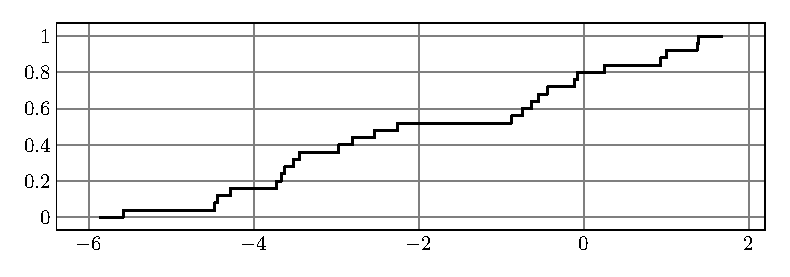
\includegraphics[scale=1]{images/st.1.eps}
  \caption{Эмпирическая функция распределения выборки 1.}\label{pic1}
\end{figure}

\begin{figure}[h]
  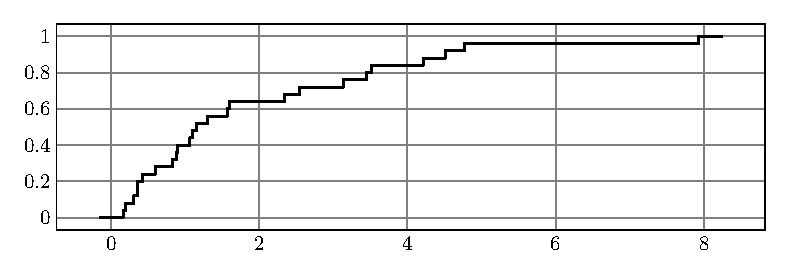
\includegraphics[scale=1]{images/st.2.eps}
  \caption{Эмпирическая функция распределения выборки 2.}\label{pic2}
\end{figure}

\par
Гистограмма относительных частот является ступенчатым приближением 
плотности распределения случайной величины $\xi$. Для ее построения 
разделим весь диапазон наблюдений на $s$ полуинтервалов вида 
$[a_{j-1}; a_j)$ и определим количество наблюдений $m_j$, попавших в 
$j$-й в полуинтервал. Относительная частота наблюдений, попавших 
в $j$-й полуинтервал, равна $P_j^* = \dfrac{m_j}{n}$. 
Так как $m_1 + \cdots + m_s = n$, то сумма всех частот равна единице: 
$\sum\limits_{j=1}^{s} P_j^* = \sum\limits_{j=1}^{s} \dfrac{m_j}{n} = 
\dfrac{1}{n} \cdot \sum\limits_{j=1}^{s} m_j = \dfrac{1}{n} \cdot n = 1$.
Над каждым полуинтервалом $j$ построим прямоугольник высоты 
$h_j = \dfrac{m_j}{n(a_j-a_{j-1})}$. Полученная фигура, состоящая 
из этих прямоугольников, называется гистограммой относительных частот. 
Ее площадь должна быть равна единице. Соответственно, площадь каждого 
прямоугольника равна относительной частоте наблюдений $P_j^*$, 
попавших в этот интервал.

\par
Для построения гистограмм следует сгруппировать данные выборок. 
Для этого разобъем область данных на несколько интервалов равной длины. 
Для первой выборки длину интервала $[a_{j-1}; a_j)$ возьмем равной 
 $1{,}4$, за $a_0$ возьмем 
минус $6$. 
Для второй выборки длину интервала $[a_{j-1}; a_j)$ возьмем равной 
 $1{,}6$, за $a_0$ возьмем 
 $0{,}0$. 
Вычислим относительные частоты попадания в эти интервалы (табл.~\ref{tab:3} 
и~\ref{tab:4}) и над каждым из них построим столбец соответствующей высоты 
(рис.~\ref{pic3} и~\ref{pic4}).

\begin{table}[h]
  \begin{minipage}[h]{0.49\linewidth}
    \caption{Выборка 1, относительные частоты.}\label{tab:3}
  \end{minipage}
  \begin{minipage}[h]{0.49\linewidth}
    \caption{Выборка 2, относительные частоты.}\label{tab:4}
  \end{minipage}
  \begin{minipage}[t]{0.49\linewidth}
  \begin{center}
    \begin{tabular}{|c|c|}
      \hline
      Интервал & Отн. частота \\
      \hline 
      
        $[-6; -4{,}6)$ & $0{,}0285714285714286$ \\
        \hline
      
        $[-4{,}6; -3{,}2)$ & $0{,}228571428571429$ \\
        \hline
      
        $[-3{,}2; -1{,}8)$ & $0{,}114285714285714$ \\
        \hline
      
        $[-1{,}8; -0{,}4)$ & $0{,}142857142857143$ \\
        \hline
      
        $[-0{,}4; 1{,}0)$ & $0{,}114285714285714$ \\
        \hline
      
        $[1{,}0; 2{,}4)$ & $0{,}0857142857142857$ \\
        \hline
      
    \end{tabular}
  \end{center}
\end{minipage}
  \hfill
  \begin{minipage}[t]{0.49\linewidth}
    \begin{center}
      \begin{tabular}{|c|c|}
        \hline
        Интервал & Отн. частота \\
        \hline 
        
          $[0{,}0; 1{,}6)$ & $0{,}375$ \\
          \hline
        
          $[1{,}6; 3{,}2)$ & $0{,}1$ \\
          \hline
        
          $[3{,}2; 4{,}8)$ & $0{,}125$ \\
          \hline
        
          $[4{,}8; 6{,}4)$ & $0{,}0$ \\
          \hline
        
          $[6{,}4; 8{,}0)$ & $0{,}025$ \\
          \hline
        
      \end{tabular}
    \end{center}
  \end{minipage}
\end{table}

\par
На основании построенных гистограмм следует выдвинуть и проверить ряд 
статистических гипотез о виде и параметрах распределения обеих случайных 
величин.

\begin{figure}[t]
  \includegraphics[scale=1]{images/st.3.eps}
  \caption{Гистограмма относительных частот выборки 1.}\label{pic3}
\end{figure}

\begin{figure}[t]
  \includegraphics[scale=1]{images/st.4.eps}
  \caption{Гистограмма относительных частот выборки 2.}\label{pic4}
\end{figure}

\par



Из построенных гистограмм видно, что из трех гипотез о нормальном, 
равномерном и экспоненциальном распределении для первой выборки наиболее 
правдоподобна гипотеза о равномерном, а для второй~--- 
экспоненциальном распределении. Дополнительные основания 
для принятия решения в каждом случае даст построение так называемых 
вероятностных бумаг.


\par
Дадим определение вероятностной бумаге. Предположим, что закон теоретической 
функции распределения известен (например, нормальное, экспоненциальное или 
равномерное распределение), но неизвестны параметры этого распределения. 
Нормальное и равномерное распределения определяются двумя параметрами 
$\alpha$ и $\beta$~--- математическим ожиданием и среднеквадратичным 
отклонением, а экспоненциальное распределение одним параметром $\lambda$~---
математическим ожиданием. Тогда теоретическую функцию распределения можно 
рассматривать как зависящую от переменной $x$ и соответствующих параметров: 
$F = F(x, \alpha, \beta)$ или $F = F(x, \lambda)$. Выберем такую систему 
координат $u = u(x)$, $v = v(x)$, чтобы график теоретической функции 
распределения в новых координатах $(u, v)$ стал прямой линией $v = ku+b$ 
с коэффициентами $k$ и $b$, зависящими от неизвестных параметров $\alpha$ 
и $\beta$: $k = \varphi(\alpha, \beta)$, $b = \psi(\alpha, \beta)$. 
Для экспоненциального распределения существует такая система координат,
в которой уравнение прямой имеет вид $v = ku$, где $k = \varphi(\lambda)$.

\par
Поскольку эмпирическая функция распределения $y = F_\text{э}(x)$ при 
достаточно большом объеме выборки лежит вблизи от теоретической функции 
рапределения $y = F(x, \alpha, \beta)$ (или при экспоненциальном 
распределении $y = F(x, \lambda)$), то после замены переменных 
график эмпирической функции должен лежать вблизи искомой прямой. 
Новая система координат $(u, v)$ с нанесенными соответствующими 
значениями $(x, y)$, преобразованными в новые координаты, называется 
вероятностной бумагой. Построив в новых координатах график эмпирической 
функции распределения, подбирают и скомую прямую так, чтобы по обе 
стороны от нее находилось примерно одинаковое количество <<ступенек>> 
построенного графика (это можно делать произвольно, а можно 
воспользоваться, например методом наименьших квадратов). Затем определяют 
$k$~--- величину тангенса угла, образованного этой прямой с осью $Ou$, 
и $b$~--- координату пересечения с осью $Ov$. Приравняв полученные величины 
к $\varphi(\alpha, \beta)$ и $\psi(\alpha, \beta)$, находят оценки 
неизвестных параметров $\alpha$ и $\beta$ из системы уравнений:

$$ 
\begin{cases}
 k = \varphi(\alpha, \beta),\\
 b = \psi(\alpha, \beta).
\end{cases} 
$$

\par
Если неизвестный параметр один (в случае экспоненциального распределения), то 
уравнение будет единственным.

\par
Для нормального закона распределения 
$$  
	F(x, m, \sigma) = \Phi \left( \frac{x-m}{\sigma} \right)  + 0.5,
$$
где $ \Phi(x) = \frac{1}{\sqrt{2 \pi}} \int\limits_{0}^{x} {e^{-\frac{x^2}{2}}} dx$ --- функция Лапласа. Сделаем следующую
замену координат:
$$  
	u = x{,} v = \Phi^{-1}(y-0.5),
$$
где $ x = \Phi^{-1}(y) $ --- функция, обратная к функции Лапласа. В новых координатах $ (u;v) $ уравнение функции распределения $ y = \Phi(\frac{x-m}{\sigma}) + 0.5, $ примет следующий вид:
$$  
	v = \Phi^{-1}(y-0.5) = \Phi^{-1}\left( \Phi \left( \frac{x-m}{\sigma} \right)  + 0.5 - 0.5\right)  = 
$$
$$
	= \Phi^{-1}\left( \Phi \left( \frac{x-m}{\sigma} \right)\right)  = \frac{x-m}{\sigma} = \frac{u-m}{\sigma}.
$$
Получившееся уравнение $ v = \dfrac{u-m}{\sigma} = \dfrac{1}{\sigma} u + (-\dfrac{m}{\sigma})  $
есть уравнение искомой прямой линии. Отсюда

$$
\left\{
\begin{array}{rcl}
k&=&\dfrac{1}{\sigma}\\
b & = &-\dfrac{m}{\sigma}.\\
\end{array}
\right.
\Longleftrightarrow
\left\{
\begin{array}{rcl}
\sigma&=&\dfrac{1}{k}\\
m & = &-\dfrac{b}{k}.\\
\end{array}
\right.
$$

Теоритическая функция распределения экспоненциально распределенной случайной величины имеет вид:

$$
y = F(x, \lambda) =\begin{cases}
1 - e^{- \lambda x},&\text{если $x \geq 0$;}\\
0,&\text{иначе.}\\
\end{cases}
$$

Здесь применяют следующую замену координат: 
$$  
	u = x{,} v = -\ln(1-y).
$$
В новых координатах уравнение теоритической функции распределения $ y = F(x,\lambda) $ примет такой вид:


$$
	v = -\ln(1-y) = -\ln(1-F(x,\lambda)) = -\ln(1-(1-e^{- \lambda x})) = -\ln(e^{- \lambda x}) = \lambda x = \lambda u \text{ } (u \geq 0).
$$

Заметим, что прямая $ v = \lambda u $ должна проходить через начало координат.

Для равномерного распределения имеем следующую теоритическую функцию 
распределения случайной величины:

$$
y = F(x,\alpha,\beta) = \begin{cases}
1,&\text{если $x > \beta$;}\\
\frac{x-\alpha}{\beta-\alpha},&\text{если $x \in [\alpha,\beta]$;}\\
0,&\text{иначе.}\\
\end{cases}
$$

Данная функция уже имеет линейный вид, поэтому можно обойтись тождественным 
преобразованием координат $u = x$, $v = y$. При этом для равномерного 
распределения известны следующие выражения для математического ожидания 
и среднеквадратичного отклонения:

$$
\left\{
\begin{array}{rcl}
m&=&\frac{\alpha+\beta}{2}\\
\sigma&=&\frac{\beta-\alpha}{2\sqrt{3}}.\\
\end{array}
\right.
$$

Имея на вероятностной бумаге линию $kx+b$, исходя из этого, параметры 
распределения можно оценить следующим образом:

$$
\left\{
\begin{array}{rcl}
\alpha&=&-\frac{b}{k}\\
\beta&=&\frac{1-b}{k}.\\
\end{array}
\right.
\Longleftrightarrow
\left\{
\begin{array}{rcl}
m&=&\frac{1-2b}{2k}\\
\sigma&=&\frac{1}{2k\sqrt{3}}.\\
\end{array}
\right.
$$

Для каждой выборки построим вероятностные бумаги равномерного, нормального и 
экспоненциального распределений (для выборки 1~--- 
рис.~\ref{pic5},~\ref{pic6} и~\ref{pic7}, 
для выборки 2~--- рис.~\ref{pic8},~\ref{pic9} и~\ref{pic10}).

\begin{figure}[h]
  \includegraphics[scale=1]{images/st.7.eps}
  \caption{Равномерная вероятностная бумага для выборки 1.}\label{pic5}
\end{figure}

\begin{figure}[h]
  \includegraphics[scale=1]{images/st.5.eps}
  \caption{Нормальная вероятностная бумага для выборки 1.}\label{pic6}
\end{figure}

\begin{figure}[h]
  \includegraphics[scale=1]{images/st.6.eps}
  \caption{Экспоненциальная вероятностная бумага для выборки 1.}\label{pic7}
\end{figure}

\begin{figure}[h]
  \includegraphics[scale=1]{images/st.10.eps}
  \caption{Равномерная вероятностная бумага для выборки 2.}\label{pic8}
\end{figure}

\begin{figure}[h]
  \includegraphics[scale=1]{images/st.8.eps}
  \caption{Нормальная вероятностная бумага для выборки 2.}\label{pic9}
\end{figure}

\begin{figure}[h]
  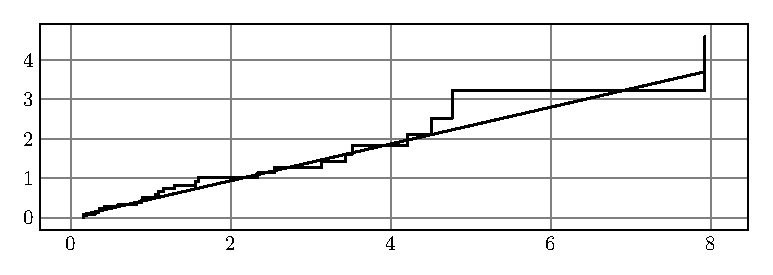
\includegraphics[scale=1]{images/st.9.eps}
  \caption{Экспоненциальная вероятностная бумага для выборки 2.}\label{pic10}
\end{figure}



\par

  
  
  
  График эмпирической функции распределения выборки $1$ наилучшим образом 
  приближается прямой на равномерной вероятностной бумаге (рис.~\ref{pic5}).
  Оценим параметры распределения выборки 1. Аппроксимирующая прямая $y = kx + b$ 
  выбрана так, что имеет параметры $k = 0{,}1387$ и 
  $b = 0{,}7307$.
  Откуда $\sigma = \dfrac{1}{2\sqrt{3}k} \approx 
  2{,}0807$ и 
  $m = \dfrac{1 - 2b}{2k} \approx -1{,}6632$.


\par

  
  
  
  Для выборки $2$ удалось подобрать прямую для вероятностной бумаги 
  экспоненциального распределения, проходящую через начало координат, 
  которая приближает эмпирическую функцию распределения выборки $2$ лучше, 
  чем прямые на других вероятностных бумагах. Поэтому, предположим, 
  что выборка $2$ имеет экспоненциальное рапределение и оценим его параметры.
  Прямая на вероятностной бумаге (рис.~\ref{pic10}) имеет параметры 
  $k = 0{,}467$ и $b = 0$, соответственно 
  параметр распределения $\lambda = 0{,}467$.



\newpage



\par
{\em Вывод.} На основании построенных гистограмм относительных частот и анализа 
равномерной, нормальной и экспоненциальной вероятностных бумаг можно выдвинуть 
гипотезы о равномерном распределении выборки 1 с параметрами 
$\sigma = 2{,}0807$ и 
                      $m = -1{,}6632$, и экспоненциальном распределении выборки 2 
с параметрами $\lambda = 0{,}467$. 

\endinput
